\documentclass[english]{beamer}

% Math
\usepackage{amssymb}
\usepackage{amsmath}
\usepackage{amsfonts}
\allowdisplaybreaks{}           % Allow pagebreaks in math environments.
\makeatletter
\g@addto@macro\bfseries{\boldmath} % Typeset bold math in headings.
\makeatother

% Font
\usepackage[utf8]{inputenc}
\usepackage[T1]{fontenc}
\usepackage{babel}
\usepackage{newpxtext}
\usepackage{newpxmath}
\usepackage{microtype}
\usepackage[autostyle=true,danish=quotes]{csquotes}
\MakeOuterQuote{"}

% Captions
\usepackage[small,hang,bf,margin=30pt]{caption}

% Graphics
\usepackage{graphicx}
\usepackage{subcaption}
\usepackage{float}
\usepackage{tikz}
\usepackage{pgfplots}
% \usetikzlibrary{external}
% \tikzexternalize[prefix=tikz/,mode=list and make]
\pgfkeys{/pgf/images/include external/.code=\includegraphics{#1}} % Makes
                                                                  % externalize
                                                                  % and draft
                                                                  % work
                                                                  % together.
\pgfplotsset{%
  invoke before crossref tikzpicture={\tikzexternaldisable},
  invoke after crossref tikzpicture={\tikzexternalenable},
  ylabel near ticks,
  legend columns=-1,
  legend style={at={(0.5, 1)},anchor=south,draw=none,fill=none,/tikz/every even
    column/.append style={column sep=10pt}},
  every y tick scale label/.style={at={(0,1)},anchor=east, font=\scriptsize,
    inner xsep=2pt, inner ysep=0pt},
  ytick placement tolerance=-2mm,
  max space between ticks=30pt,
}
\usetikzlibrary{arrows}
\usepgfplotslibrary{groupplots}

% Fixme
\usepackage[draft]{fixme}

% Colors
\usepackage{color}
\definecolor{my-red}{HTML}{E41A1C}
\definecolor{my-green}{HTML}{4DAF4A}
\definecolor{my-blue}{HTML}{377EB8}
\definecolor{my-purple}{HTML}{984EA3}
\definecolor{my-orange}{HTML}{FF7F00}

% User defined macros
\DeclareMathOperator*{\argmin}{arg\,min}
\DeclareMathOperator*{\argmax}{arg\,max}

% Date
\usepackage{datetime}

% Beamer stuff.
\usetheme{default}
\setbeamertemplate{navigation symbols}{}
\AtBeginSection[]
{
 \begin{frame}<beamer>
 \frametitle{Plan}
 \tableofcontents[currentsection]
 \end{frame}
}

% Symbols
\usepackage[weather]{ifsym}

\title{Speeding Up HMM Decoding Using Compression}
\author{Torben Muldvang Andersen, 20093713}
\date{\protect\formatdate{24}{06}{2015}}

\begin{document}
\begin{frame}
  \maketitle
  
\includegraphics[height=7mm, trim=0 0 40mm 0, clip]{../logo}
  \hfill
  
\includegraphics[height=7mm]{../BiRC-logo}
\end{frame}

\begin{frame}
  \frametitle{Agenda}
    Med udgangspunkt i specialerapporten ønskes et foredrag, hvor de
    væsentligste resultater af specialeprojektet fremlægges.
  \begin{itemize}
  \item Du bedes presentere hvorledes skjulte Markov modeller anvendes til
    Viterbi- og Posterior-decoding med fokus på hvorledes implementeringen af
    disse decoding-methoder kan formuleres ved hjælp af lineær algebra samt
    hvorledes en præprocessesing med henblik på en ``komprimering'' af input
    kan forbedre deres kørselstid i praksis.
  \item Du bedes også præsentere dine implementeringer af metoderne og
    udvidelser til biblioteket zipHMMlib samt de eksperimenter som du har
    gennemført for at undersøge deres kørselstider i praksis, herunder hvornår
    præprocesseringen giver den ønskede forbedring af kørselstiden.
  \item Endelig bedes du overveje hvorvidt andre former for præprocessering
    (komprimering) kunne anvedes.
  \end{itemize}
\end{frame}

\begin{frame}
  \frametitle{Agenda}
  \tableofcontents{}
\end{frame}

\section{Hidden Markov Models}

\begin{frame}
  \frametitle{\insertsection}
  \begin{columns}
    \begin{column}{0.5\textwidth}
      \onslide<2->
      \begin{itemize}
      \item Hidden states: L, H.
      \item Observables: \Sun, \Cloud, \Rain.
      \end{itemize}
    \end{column}%
    \begin{column}{0.5\textwidth}
      \onslide<1->
      \begin{figure}
        \centering \tikzsetnextfilename{HMM}
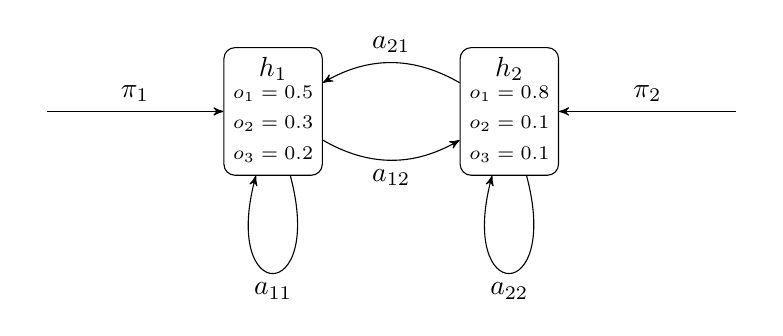
\begin{tikzpicture} [
  ->,
  >=stealth',
  auto,
  node distance=3cm,
  main node/.style={rectangle,draw,rounded corners,align=center},
  ]

  \node[main node] (h1) {$h_1$\\{\scriptsize%
    $\begin{aligned}
        o_1 &= 0.5\\ o_2 &= 0.3\\ o_3 &= 0.2\\
    \end{aligned}$}};
  \node[main node, right of=h1] (h2) {$h_2$\\{\scriptsize%
    $\begin{aligned}
        o_1 &= 0.8\\ o_2 &= 0.1\\ o_3 &= 0.1\\
    \end{aligned}$}};
  \node[left of=h1] (p1) {};
  \node[right of=h2] (p2) {};

  \path
    (h1) edge[bend right]               node[below] {$a_{12}$} (h2)
         edge[loop below, looseness=10] node        {$a_{11}$} (h1)
    (h2) edge[bend right]               node[above] {$a_{21}$} (h1)
         edge[loop below, looseness=10] node        {$a_{22}$} (h2);

  \path
    (p1) edge node[above] {$\pi_1$} (h1)
    (p2) edge node[above] {$\pi_2$} (h2);
\end{tikzpicture}

%%% Local Variables:
%%% mode: latex
%%% TeX-master: "../master"
%%% End:

      \end{figure}
    \end{column}
  \end{columns}
  \begin{center}
    \begin{tabular}{cccccccccc}
      \onslide<3-> \Sun & \Sun & \Sun & \Cloud & \Cloud & \Rain & \Rain & \Sun & \Sun & \Sun \\
      \onslide<4-> H    & H    & H    & H      & L      & L     & L     & L    & H    & H    \\
    \end{tabular}
  \end{center}
  \begin{itemize}
    \tiny
  \item Very short introduction using figure from thesis.
  \item Example with observation sequence. How come? Informal definition of
    Viterbi decoding.
  \item Simple explanation of Viterbi decoding using weather example and figure.
    Perspectivation to bioinformatics.
  \end{itemize}
\end{frame}

\section{Viterbi Decoding}

\subsection{The Original Viterbi Algorithm}

\begin{frame}
  \frametitle{\insertsubsection}
  \begin{itemize}
    \tiny
  \item Definition.
  \item Dynamic programming table.
  \item Backtracking.
  \item Assymptotic running time and some perspectivation to bioinformatics.
  \end{itemize}
\end{frame}

\subsection{Linear Algebra}

\begin{frame}
  \frametitle{\insertsubsection}
  \begin{itemize}
    \tiny
  \item Reformulation. (Would be really cool if this could be made using an
    illustration of the stuff multiplied in the original algorithm and the
    table using the weather example.)
  \item Running time.
  \end{itemize}
\end{frame}

\subsection{Exploting Repetitions}

\begin{frame}
  \frametitle{\insertsubsection}
  \begin{itemize}
    \tiny
  \item Example of byte-pair encoding on weather example.
  \item Continue example on the illustration of table.
  \item Backtracking.
  \item Running time.
  \end{itemize}
\end{frame}

\section{Posterior Decoding}

\begin{frame}
  \frametitle{\insertsection}
  \begin{itemize}
    \tiny
  \item Definition.
  \item Definition of forward-backward algorithm (compare to Viterbi)
  \item Exploiting repetitions similarly to Viterbi.
  \item Backtracking.
  \end{itemize}
\end{frame}

\section{Indexed Posterior Decoding}

\begin{frame}
  \frametitle{\insertsection}
  \begin{itemize}
    \tiny
  \item Definition.
  \item Illustration using figure from thesis.
  \end{itemize}
\end{frame}

\section{Implementation}

\begin{frame}
  \frametitle{\insertsection}
  \begin{itemize}
    \tiny
  \item Something about the implementation.
  \end{itemize}
\end{frame}

\section{Experiments}

\begin{frame}
  \frametitle{\insertsection}
  \begin{itemize}
    \tiny
  \item Main experiments.
  \item Some kind of summary of experiments
  \end{itemize}
\end{frame}

\section{Other Types of Preprocessing}

\begin{frame}
  \frametitle{\insertsection}

\end{frame}
\end{document}



%%% Local Variables:
%%% mode: latex
%%% TeX-master: t
%%% End:
